\documentclass{article}
\usepackage[T1]{fontenc}
\usepackage{times}
\usepackage{xcolor}
\usepackage{pgfplots}
% Shared publication style for every quantitative and conceptual figure.
% Color semantics are fixed across the paper:
%   blue = balanced / position-robust behavior
%   coral = confounded / shortcut-sensitive behavior
%   sand = transition or intermediate state
%   gray = reference or secondary diagnostic
\definecolor{fig-balanced}{HTML}{4E8D96}
\definecolor{fig-confounded}{HTML}{C96F5F}
\definecolor{fig-transition}{HTML}{D8C58D}
\definecolor{fig-neutral}{HTML}{8C8C96}
\definecolor{fig-ink}{HTML}{303840}
\definecolor{fig-light}{HTML}{F4F7F8}

\usetikzlibrary{arrows.meta,positioning,calc}
\pgfplotsset{
    compat=1.18,
    expplot/.style={
        width=\columnwidth,
        tick label style={font=\footnotesize, text=fig-ink},
        xlabel style={font=\footnotesize, text=fig-ink},
        ylabel style={font=\footnotesize, text=fig-ink},
        legend style={font=\footnotesize, draw=none, cells={anchor=west}},
        every axis plot/.append style={line width=1.0pt, mark size=2.6pt},
        tick style={draw=fig-ink, line width=0.45pt},
        axis line style={draw=fig-ink, line width=0.55pt},
        axis lines=left,
    },
    expgrid/.style={
        ymajorgrids=true,
        grid style={draw=fig-neutral!18, line width=0.4pt},
    },
}


\begin{document}
\pagestyle{empty}
\setbox0=\hbox{%
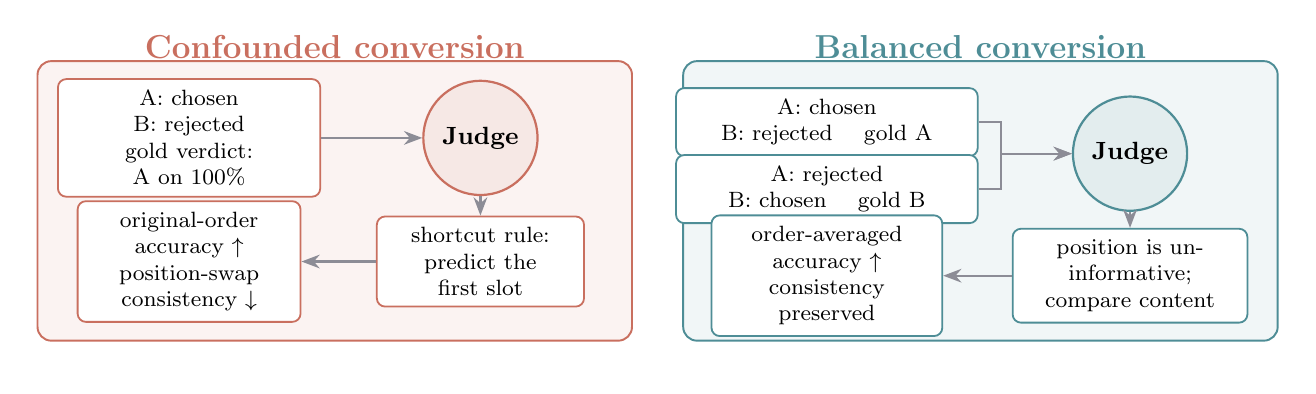
\begin{tikzpicture}[
    font=\footnotesize,
    >=Stealth,
    panel/.style={rounded corners=5pt, line width=0.7pt, minimum width=7.55cm, minimum height=3.55cm},
    card/.style={rounded corners=3pt, fill=white, line width=0.65pt, align=center, inner sep=4pt},
    judge/.style={circle, minimum size=1.45cm, line width=0.8pt, align=center, font=\bfseries\small},
    flow/.style={-Stealth, draw=fig-neutral, line width=0.8pt},
]
\path[use as bounding box] (-0.05,-0.05) rectangle (15.95,4.25);

\node[font=\bfseries\large, text=fig-confounded] at (3.85,4.00) {Confounded conversion};
\node[panel, draw=fig-confounded, fill=fig-confounded!8] at (3.85,2.05) {};
\node[card, draw=fig-confounded, text width=3.05cm] (ldata) at (2.00,2.85)
    {A: chosen \quad B: rejected\\gold verdict: A on 100\%};
\node[judge, draw=fig-confounded, fill=fig-confounded!16] (ljudge) at (5.70,2.85) {Judge};
\node[card, draw=fig-confounded, text width=2.35cm] (lrule) at (5.70,1.28)
    {shortcut rule:\\predict the first slot};
\node[card, draw=fig-confounded, text width=2.55cm] (lout) at (2.00,1.28)
    {original-order accuracy $\uparrow$\\position-swap consistency $\downarrow$};
\draw[flow] (ldata.east) -- (ljudge.west);
\draw[flow] (ljudge.south) -- (lrule.north);
\draw[flow] (lrule.west) -- (lout.east);

\node[font=\bfseries\large, text=fig-balanced] at (12.05,4.00) {Balanced conversion};
\node[panel, draw=fig-balanced, fill=fig-balanced!8] at (12.05,2.05) {};
\node[card, draw=fig-balanced, text width=3.55cm] (rdataa) at (10.10,3.05)
    {A: chosen \quad \mbox{B: rejected} \quad gold A};
\node[card, draw=fig-balanced, text width=3.55cm] (rdatab) at (10.10,2.20)
    {A: rejected \quad \mbox{B: chosen} \quad gold B};
\node[judge, draw=fig-balanced, fill=fig-balanced!16] (rjudge) at (13.95,2.65) {Judge};
\node[card, draw=fig-balanced, text width=2.70cm] (rrule) at (13.95,1.10)
    {position is uninformative;\\compare content};
\node[card, draw=fig-balanced, text width=2.65cm] (rout) at (10.10,1.10)
    {order-averaged accuracy $\uparrow$\\consistency preserved};
\draw[flow] (rdataa.east) -- ++(0.28,0) |- (rjudge.west);
\draw[flow] (rdatab.east) -- ++(0.28,0) |- (rjudge.west);
\draw[flow] (rjudge.south) -- (rrule.north);
\draw[flow] (rrule.west) -- (rout.east);
\end{tikzpicture}
}%
\pdfpagewidth=\wd0
\pdfpageheight=\dimexpr\ht0+\dp0\relax
\hoffset=-1in
\voffset=-1in
\shipout\box0
\end{document}
